\documentclass[10pt]{article}
\usepackage{icmlko}

\icmlmeta{IP 파운데이션 월드모델}{483}{합류점이 없었다 --- 그리고 남은 신호의 이름은 시각이다}{크로스 어텐션을 짓기 전에 강 양쪽을 세었다. 다리는 0개였고, 강물의 78\%는 입력과 무관한 상수였다}

\begin{document}

\twocolumn[
\icmlheader

\begin{abstract}
사용자가 요구한 것은 \textbf{개입 $\to$ 변화}의 월드모델이다 --- 정보전이장
$g(x,t)$ 를 인코딩하는 인코더를 따로 두고, 이벤트 인코더와 \emph{``크로스 어텐션
같은''} 합류로 잇는 구조. 그리고 \emph{``꼭 크로스 어텐션일 필요는 없고 좋은
아키텍처를 계속 연구해 보라''}.

\textbf{그래서 짓기 전에 세었다.} 저장소의 파이썬 \textbf{604개}를 전수 AST 로
훑어 조각이 서로 닿는지 셌다. 결과는 \textbf{다리 0개}다 --- 장 인코더와 텍스트
인코더를 \emph{함께 반입하는 파일이 하나도 없고}, 장 인코더와
\texttt{shared\_encoder}/\texttt{foundation} 을 잇는 경로도 없으며,
\texttt{state/} 의 조각 \textbf{넷}(\texttt{shared\_encoder} ·
\texttt{masked\_encoder} · \texttt{transfer\_eval} · \texttt{fewshot})은
\textbf{아무도 안 부른다}. 이 저장소에 실재하는 유일한 합류는
\textbf{GBDT 특성 행렬에 열을 나란히 놓는 것}이고, 두 축 이름
(\texttt{field\_spread\_ff} · \texttt{text\_nn})이 함께 나오는 파일은 --- 이 진단을
위해 오늘 내가 쓴 파일 하나를 빼면 --- \textbf{0개}다.

\textbf{그리고 합류할 값이 있는지 쟀다.} 얼린 장 인코더의 표현
($\mathrm{dim}=4$ 를 동네 축으로 눌러 평균·산포 8열)이 학습에서 배운 방향을 유보에서
얼마나 지키나: $S=\mathbf{+0.0508}$ 로 현행 1열 축($+0.0112$)의 \textbf{4.5배}다.
퇴화 도메인 넷(유보 고유날 $<10$)을 빼면 $+0.0738$ 이고 날짜 군집 BCa 하한이
$+0.0095$ 로 0 을 안 문다. \textbf{1열로 눌러서 잃는 것이 실재한다.}

\textbf{그런데 그 남은 것의 이름이 시각이었다.} 표준화한 \textbf{날짜 한 열}이
$S=\mathbf{+0.1149}$ (BCa $\lbrack+0.065,+0.184\rbrack$) 로 장의 표현 8열을
\textbf{1.6배} 이긴다.
장이 시각 위에 더하는 증분은 $\Delta S = \mathbf{+0.0094}$ 이고 순열 널 $2\sigma$
$0.0392$ 의 \textbf{0.24배}다 --- \textbf{널 안이다.}

\textbf{왜인지도 잡았다.} 학습 규율의 NN 판본(\texttt{docs/아키텍처.md} §9.1)을
얼린 인코더에 돌렸더니, \texttt{mix} 로 들어가는 세 갈래 중
\textbf{동네 임베딩을 0 으로 만들면 표현이 77.8\% 바뀌고} 정작 \textbf{입력 창을
0 으로 만들면 9.8\%}, 이웃 혼합은 \textbf{4.0\%} 만 바뀐다. \textbf{표현의 대부분이
입력과 무관한 상수 조회표}다.

\textbf{그래서 2단계(합류 구조 겨루기)를 열지 않는다.} 그리고 판정을 못 낸 이유가
하나 더 있다 --- \textbf{내 사전등록 규칙이 두 군데 틀렸다.} 실측이 떨어진 자리를
어느 규칙도 안 덮었고(노트 756 의 구멍, \textbf{세 번째}), 위약 규칙은 부호를 안 봐서
\textbf{널 폭을 교란으로 오인해 발동}했다.
\end{abstract}
]

\section{0단계 --- 조각은 있는데 다리가 없다}

지시는 \emph{``읽고 세기 전에 아무것도 짓지 마라''} 였다. 셌다.

\subsection{연결을 눈으로 읽지 않았다}

\texttt{runners/wire897.py} 가 저장소의 \texttt{.py} \textbf{604개}를 AST 로 파싱해
\texttt{import}/\texttt{from} 을 전수 수집하고 역방향 색인을 만든다. 상대 반입은
패키지 경로로 풀었다. 결과가 표 \ref{tab:graph} 이고 그림 \ref{fig:1}(a) 다.

\begin{table}[h]\centering\tsize
\begin{tabular}{lr}
\toprule
조각 & 반입하는 파일 수 \\
\midrule
\texttt{lab.forms} & 118 \\
\texttt{lab.harness} & 73 \\
\texttt{state.tri\_domain} & 36 \\
\texttt{state.fieldmodel} & 14 \\
\texttt{state.slots} & 10 \\
\texttt{lab.textnn} & 7 \\
\texttt{lab.joint} & 1 \\
\texttt{state.encoder} & 1 \\
\texttt{state.foundation} & 1 \\
\midrule
\texttt{state.shared\_encoder} & \textbf{0} \\
\texttt{state.masked\_encoder} & \textbf{0} \\
\texttt{state.transfer\_eval} & \textbf{0} \\
\texttt{state.fewshot} & \textbf{0} \\
\bottomrule
\end{tabular}
\caption{조각별 호출자 수. 아래 넷은 \texttt{\_\_main\_\_} 스크립트로 한 번 돌고
\texttt{data/state/*.json} 을 남긴 뒤 \textbf{어떤 파이프에도 안 붙었다}.}
\label{tab:graph}
\end{table}

\claimx{\textbf{장 인코더 출력이 \texttt{shared\_encoder}/\texttt{foundation}
파이프에 닿는 경로는 없다.} 교집합 \textbf{0개}. 더 세게, \textbf{장 인코더와 텍스트
인코더를 함께 반입하는 파일도 0개}이고, 두 축 이름이 함께 나오는 파일도 (이 진단
파일을 빼면) \textbf{0개}다. 이 저장소가 아는 유일한 합류는 \textbf{GBDT 특성 행렬의
열 나열}이며 그것조차 두 인코더로 동시에 해 본 적이 없다.}
{저 넷 중 하나라도 \texttt{lab/} 파이프에서 반입되는 곳이 발견되면 이 주장은
틀린다. AST 가 못 보는 동적 반입(\texttt{importlib} · 문자열 경유)이 있으면
같이 틀린다 --- 산출물에 파일 목록을 전량 실어 두었다.}

\subsection{돌려 봤다 --- 그리고 시간초과는 셋째 범주다}

조각을 실제로 돌렸다(\texttt{runners/inv897.py}). \textbf{종료 코드 0 을 성공으로
읽지 않고} 표준출력의 \emph{내용}으로 판정한다(조항 59). 초판은 상한을 30분으로
뒀는데 \texttt{state.shared\_encoder} 가 그 30분을 통째로 태우고 아무것도 안
냈다 --- \texttt{docs/아키텍처.md} §4 의 \emph{``팔 하나가 10분을 넘으면 사다리를
줄여라''} 를 따라 상한을 300초로 내리고 \textbf{「300초 안에 안 끝난다」를 결과로}
적는다.

\begin{table}[h]\centering\tsize
\begin{tabular}{lrrl}
\toprule
조각 & 초 & 종료 & 내용 판정 \\
\midrule
\texttt{fieldmodel horizons} & 1.2 & 0 & 돈다 (지평 8개) \\
\texttt{foundation} & 158.8 & 0 & 돈다 \\
\texttt{masked\_encoder} & 80.7 & 0 & 돈다 \\
\texttt{fewshot} & 8.4 & 0 & 돈다 \\
\texttt{transfer\_eval} & 2.7 & 0 & 돈다 \\
\texttt{shared\_encoder} & 300.0 & --- & \textbf{300초 안에 안 끝난다} \\
\texttt{encoder} & 0.7 & \textbf{0} & \textbf{출력 0바이트} \\
\bottomrule
\end{tabular}
\caption{0단계 실행. \textbf{`돈다' · `이 상한 안에 안 끝난다' · `종료 0 인데 아무것도
안 한다'는 셋이다.}}
\label{tab:run}
\end{table}

\claimx{\textbf{\texttt{state.encoder} 는 종료 코드 0 을 내면서 0바이트를 낸다.}
\textbf{그런데 이것을 「고장」으로 읽으면 안 된다}(조항 59 --- 빈 것을 부정으로 읽지
마라). 읽어 보면 \texttt{main()} 이 \texttt{--train}/\texttt{--pretrain}/%
\texttt{--transfer} 플래그가 있을 때만 무언가를 하고, 없으면 \texttt{return 0} 이다.
\textbf{`고장'이 아니라 `인자 없이는 아무 일도 안 한다'} 이고, 이 둘을 가르는 유일한
길이 \textbf{출력 내용을 보는 것}이었다.}
{\texttt{--transfer} 를 주고 돌렸을 때도 0바이트면 그때는 진짜 고장이다.}

\subsection{그리고 문서가 없는 함수를 약속하고 있다}

\texttt{state/fieldmodel.py} 의 docstring 은 쓰는 법으로 세 명령을 적는다 ---
\texttt{horizons} · \texttt{pretrain} · \texttt{readout}. 그런데
\textbf{\texttt{readout} 은 이 저장소 어디에도 없다}(\texttt{grep -rn "def readout"}
$\to$ 0건). \textbf{설계 ⑤ ``읽어내기는 기존 판에 꽂는다''는 파일 안에서 구현된 적이
없고}, 대신 \texttt{runners/} 의 여섯 파일이 \texttt{Enc} 클래스를 \textbf{손으로
베껴} 각자 다시 선언한다(\texttt{ff753} · \texttt{field744} · \texttt{biz768} ·
\texttt{conv734} · \texttt{hold732} · \texttt{ship736}). 노트 702 가 \emph{``재구현이
저계수 이웃 혼합을 빠뜨려 잴 대상을 지웠다''} 를 기록해 놓고도 구조가 그대로다.

\section{1단계 --- 표현은 남는다}

\subsection{자를 새로 만들었다}

판 $\rho$ 를 안 썼다. 판 챔피언은 \texttt{HistGradientBoostingRegressor} 라 합류
구조가 들어갈 자리가 없고, 사용자가 원하는 것은 순위 예측이 아니라 개입$\to$변화다.
게다가 정본 $0.4710$ 은 오늘 재현되지 않는다(티처 \#59 C1 · 실측 $0.469823$).

\textbf{정오 --- 이 문장을 이 사이클 안에서 정정한다.} 같은 사이클의 이슈 \#112 담당이
커밋 \texttt{4156139e2} 로 정정했다: \textbf{$0.4710$ 은 오늘도 재현된다 --- 다른 자로만.}
그쪽이 보고한 원인은 잡음이 아니라 \textbf{규약 차 둘}(채점 배치 · \texttt{random\_state}
적합 경로)이고, 정본을 $0.46982$ 로 갱신하며 $0.4710$ 에 \textbf{「837 시대 값」} 딱지를
붙였다. 그러므로 옳은 문장은 \emph{``재현되지 않는다''} 가 아니라
\textbf{``챔피언 경로로는 재현되지 않고 837 경로로는 재현된다''} 이다 ---
\textbf{`안 나온다' 와 `다른 자로 나온다' 는 둘이다}(조항 59).
⚠ 그 수치는 \textbf{그쪽 산출물이고 내가 재현하지 않았다}(조항 60).
\textbf{이 사이클의 결론은 안 바뀐다} --- 판 $\rho$ 도 문턱도 자로 쓰지 않았고 새 자 $S$ 의
널을 직접 뽑았다. 자를 새로 만든 나머지 두 이유(판 챔피언이 트리다 · 원하는 것이 순위
예측이 아니라 개입$\to$변화다)는 혼자서도 충분하다.

\[
S \;=\; \frac{\sum_d n_d \cdot \mathrm{sign}(\rho^{\text{학습}}_d)\cdot
\rho^{\text{유보}}_d}{\sum_d n_d}
\]

\textbf{부호를 학습에서 고정}하므로 사후에 유리한 부호를 고를 수 없다.
$n_d$ 는 도메인 $d$ 의 유보 행수다. 널은 빌리지 않고 셋으로 직접 뽑았다 ---
유보 라벨 도메인 안 순열 \textbf{1,000회} · \textbf{날짜 군집} BCa($B{=}2{,}000$) ·
\textbf{위약 팔 셋}(행의 날짜 연결만 끊는다).

\claimx{\textbf{군집은 프랜차이즈가 아니라 날짜다.} 이 축의 특성은 \emph{날짜만의
함수}라 같은 날 행이 완전히 종속이다. 유보 3,710행이 \textbf{날짜 군집 540개}로
접힌다(병합률 \textbf{0.854}). 규약 47 의 재표집 단위(프랜차이즈)보다 날짜가 상위
군집이므로 날짜를 쓰고 병기했다. \textbf{순열 널과 군집 구간이 다른 답을 낸 이유가
정확히 이 6.9배 축소다.}}
{같은 날 행이 실제로는 독립이라면(예: 특성에 행별 성분이 있다면) 날짜 군집은
과도하게 보수적이다. 그때는 행 부트가 맞고 구간이 좁아진다.}

\subsection{노트 756 을 소수 셋째 자리까지 재현했다}

1열 팔은 노트 756 이 잰 값을 다시 내야 한다(스피어만은 전역 단조 변환에 불변).
실측: 웹툰 $+0.0816\to+0.0216$(756: $+0.082\to+0.022$) · 애니
$+0.0774\to+0.0203$($+0.077\to+0.020$) · 아이돌 $+0.1247\to+0.0464$ · 만화
$+0.0507\to-0.0259$ · 세계애니 $+0.0533\to-0.0133$ · 도서 $-0.0205\to-0.1104$ ·
시장팝업 $-0.0345\to-0.1212$ · 게임 $+0.0212\to+0.0134$ · 모바일
$-0.0169\to+0.0058$ · 펀딩 $+0.0036\to-0.0685$. \textbf{열 중 열이 일치한다.}
(팝업은 학습 24행이라 이번 최소 행수에서 빠졌고, 영화는 756 이후 붙은 12번째
도메인이다.)

\claimx{\textbf{측정 사슬이 검증됐다} --- 자료 $\to$ \texttt{field} $\to$
\texttt{enc.pt} $\to$ 축 $\to$ 도메인별 상관까지 노트 756 과 같은 값을 낸다. 그러니
아래 새 값들이 다른 사슬에서 나온 것이 아니다.}
{도메인 이름 대응이나 창 경계가 달랐다면 값이 어긋났을 것이다.}

\subsection{표현이 1열보다 4.5배 남는다}

$S(\text{1열}) = +0.0112$ (순열 널 $2\sigma$ $0.0330$ --- \textbf{널 안}) 대
$S(\text{표현 8열}) = \mathbf{+0.0508}$ (널 $2\sigma$ $0.0325$ --- \textbf{$3.1\sigma$
밖}). 날짜 군집 BCa 는 각각 $[-0.023,+0.053]$ 과 $[-0.006,+0.134]$ 로 \textbf{둘 다 0 을
문다}.

퇴화 도메인 넷(시장팝업 · 아이돌 · 영화 · 펀딩 --- 시작 시각이 연 단위라 유보
고유날이 \textbf{2})을 빼면 $S(\text{표현}) = \mathbf{+0.0738}$ 이고 BCa
$[+0.0095,+0.1699]$ 로 \textbf{0 을 안 문다}. 이 제외는 \textbf{사후}다 ---
판정에 안 쓰고 다음 사이클의 사전등록 대상으로 남긴다.

\section{그런데 남은 것의 이름이 시각이다}

\subsection{날짜 한 열이 장의 표현 8열을 이긴다}

표현 8열이 날짜와 세게 단조다(그림 \ref{fig:2}(c) --- 열별 스피어만 $+0.776$ ·
$-0.766$ · $-0.545$ · $+0.472$ · $+0.469$ · $-0.274$ · $-0.229$ · $-0.205$).
그래서 시각을 통제했다(표 \ref{tab:partial}).

\begin{table}[h]\centering\tsize
\begin{tabular}{lrrl}
\toprule
팔 & 열 & $S$ & 날짜 군집 BCa \\
\midrule
\multicolumn{4}{l}{\emph{전 도메인 ($n=3{,}710$ · 군집 540)}}\\
ㅂ-1 시각만 & 1 & $+0.0682$ & $[-0.010,+0.132]$ \\
ㅂ-3 장만 & 8 & $+0.0508$ & $[-0.006,+0.134]$ \\
ㅂ-2 시각+장 & 9 & $+0.0861$ & $[+0.016,+0.186]$ \\
\midrule
\multicolumn{4}{l}{\emph{퇴화 제외 ($n=2{,}598$ · 군집 538)}}\\
ㅂ-1 시각만 & 1 & $\mathbf{+0.1149}$ & $[+0.065,+0.184]$ \\
ㅂ-3 장만 & 8 & $+0.0738$ & $[+0.010,+0.170]$ \\
ㅂ-2 시각+장 & 9 & $+0.1243$ & $[+0.049,+0.243]$ \\
\bottomrule
\end{tabular}
\caption{시각 통제. \textbf{장의 증분} $\Delta S = $ ㅂ2 $-$ ㅂ1 $=
\mathbf{+0.0179}$(전 도메인) · $\mathbf{+0.0094}$(퇴화 제외). 같은 자리의
순열 널 $2\sigma$ 는 $0.032$ · $0.039$ 다.}
\label{tab:partial}
\end{table}

\claimx{\textbf{장의 표현이 「시각」위에 더하는 것은 널 안이다} ---
$\Delta S = +0.0094$ 대 널 $2\sigma$ $0.0392$ (\textbf{0.24배}). 그리고 \textbf{날짜
한 열이 장의 표현 8열보다 1.6배 세다}($+0.1149$ 대 $+0.0738$). 즉 표현 수준의
$+0.0738$ 은 \emph{장의 정보}가 아니라 대체로 \emph{달력}이다.}
{장의 증분이 널 $2\sigma$ 밖으로 올라오면 틀린다. 또는 시각 1열이 판의 기존
\texttt{cal\_*} 축과 중복이라 이 비교가 부당하다면 --- 그 경우 시각 팔을 판에
넣었을 때 신호 몫이 0 이어야 하고, 그것이 다음 사이클의 확인 측정이다.}

\subsection{순수 시간 기저는 반대로 죽는다 --- 그래서 자가 대칭이 아니다}

시간 RBF \textbf{8열}(표현과 열 수를 맞춘 것)은 $S = -0.0258$ 로 오히려 음수다.
같은 시간을 \textbf{1열 단조}로 주면 $+0.1003$ 이다. \textbf{원인은 외삽}이다 ---
RBF 가중이 학습 구간(2025 이전)에 몰려 있어 유보에서 꺼진다. 그러므로
\emph{``시간 8열도 안 되니 표현 8열의 값은 진짜''} 라고 읽으면 안 된다.
\textbf{옳은 대조는 단조 시각 1열이고, 그것이 이긴다.}

\section{왜 --- 표현의 78\%가 입력과 무관한 상수다}

\texttt{docs/아키텍처.md} §9.1 의 배선 검사 여덟을 얼린 인코더에 돌렸다
(\texttt{runners/nnchk897.py}). 여덟 중 \textbf{여섯을 돌렸고 하나는 이미 돌아 있었고
하나는 못 돈다}(새 블록이 없어 「항등 붕괴」는 L1 을 여는 사이클의 첫 검사로 남긴다).

\begin{itemize}\setlength\itemsep{1pt}
\item \textbf{① 한 배치 과적합 --- 통과.} 16창을 $0.0270 \to 0.000278$
(비율 $0.0103$ · 문턱 $0.05$). \textbf{배선은 안 끊겼다.}
\item \textbf{③ 층별 $\|\Delta\theta\|$ --- 죽은 층 0개.}
\textbf{④ 기울기 노름 --- NaN/Inf 0개.}
\item \textbf{⑧ 결정성 --- 비트 동일}(sha256 대조).
\item \textbf{⑥ 입력 지우기 --- 여기서 걸렸다.}
\end{itemize}

\texttt{mix} 로 들어가는 세 갈래를 하나씩 0 으로 만들고 표현이 얼마나 바뀌나:

\begin{table}[h]\centering\tsize
\begin{tabular}{lrr}
\toprule
지운 갈래 & $\|\Delta\text{표현}\|/\|\text{표현}\|$ & 1열축 스피어만 \\
\midrule
$e$ \ 동네 임베딩 & $\mathbf{0.778}$ & $0.293$ \\
$h$ \ 과거 창 사영 & $0.098$ & $0.810$ \\
$g$ \ 저계수 이웃 혼합 & $0.040$ & $0.685$ \\
\bottomrule
\end{tabular}
\caption{\textbf{동네 임베딩은 $t$ 에도 입력에도 안 의존하는 상수 조회표}인데
표현 크기의 대부분을 차지한다. 정작 관측 창은 9.8\% 다.}
\label{tab:ablate}
\end{table}

\claimx{\textbf{장 인코더의 표현은 대부분 입력과 무관한 상수다.} 동네 임베딩을
지우면 표현이 \textbf{77.8\%} 바뀌고 관측 창을 지우면 \textbf{9.8\%} 바뀐다.
이것이 「표현을 동네 축으로 눌러 판에 넣으면 남는 것이 달력뿐」인 이유의 유력한
후보다 --- \textbf{시간에 의존하는 성분이 큰 상수 위의 작은 섭동}이고, 그 섭동의
느린 표류가 곧 달력이다. \textbf{모든 갈래가 출력에 닿기는 한다}(887형 중립화 0건).}
{임베딩을 지운 뒤 \emph{다시 학습}했을 때 유보 $R^2$ 가 안 떨어지면 이 상수는
그냥 여분이고, 떨어지면 상수가 실제로 일을 하는 것이다 --- 어느 쪽이든 오늘의
$S$ 해석은 바뀐다. \textbf{이번 사이클은 재학습을 안 했다.}}

\section{판정 --- 그리고 내 규칙이 두 군데 틀렸다}

\subsection{어느 규칙도 발동하지 않았다 (노트 756 의 구멍, 세 번째)}

사전등록은 F1(널 안 \emph{그리고} BCa 가 0 을 문다) · F2(널 밖 \emph{그리고} BCa 가
0 을 안 물고 \emph{그리고} 표현 $>$ 1열) · F3(널 밖인데 표현 $\le$ 1열) 로 갈랐다.
실측은 \textbf{널 밖 + BCa 가 0 을 뭄 + 표현 $>$ 1열} 이고 \textbf{셋 어디에도
안 든다}. 그리고 나는 그 사전등록 문서 안에
\emph{``판정 규칙은 값의 전 구간을 덮는다(노트 756 의 교훈)''} 이라고 적어 두었다.

\claimx{\textbf{규칙의 구멍이 세 번째로 재발했다} --- 노트 756(6이상/4이하로 적어
5가 샜다), 노트 757 계열, 그리고 여기. \textbf{공통 원인은 「두 개의 널을 AND 로
묶으면서 둘이 어긋날 경우를 안 적은 것」}이다. \textbf{처방을 값으로 적는다: 서로 다른
널을 쓰는 조건은 반드시 $2\times2$ 표로 네 칸을 다 적는다.}}
{네 칸 중 한 칸이라도 비어 있는 사전등록이 다음 사이클에 또 나오면 처방이 안 먹은
것이다.}

\subsection{위약 규칙은 부호를 안 봐서 과잉 발동했다}

F4 는 \emph{``위약 $|S|$ 중 하나라도 진짜 $|S|$ 의 0.5배 이상이면 팔 무효''} 였다.
위약 셋은 $+0.0087$ · $\mathbf{-0.0271}$ · $+0.0130$ 이고
$0.0271/0.0508 = \mathbf{0.534} \ge 0.5$ --- \textbf{규칙대로면 F4 발동, 팔 전체
무효}다. 그런데 발동시킨 것은 \textbf{음수 위약}이고, 음의 방향으로 큰 위약은
\emph{교란}이 아니라 \textbf{널 폭}이다. 실제로 위약 셋의 흩어짐($\approx0.021$)은
순열 널 SD($0.0163$)와 같은 자릿수이고, \textbf{두 널이 서로를 확인해 준다}.

\claimx{\textbf{규칙대로 F4 를 발동시키고 팔을 무효로 적는다} --- 사후에 규칙을
고쳐 살리지 않는다. 동시에 \textbf{규칙이 잘못 적혔음을 기록한다}: 위약 문턱은
$|S|$ 가 아니라 \textbf{부호를 맞춘 $S$} 또는 \textbf{위약 분포의 SD 대비 $z$} 로
적었어야 한다. 그리고 \textbf{뽑기 셋으로 SD 를 재는 것 자체가 얇다.}}
{위약을 12뽑기로 늘렸을 때 SD 가 $0.021$ 근처로 수렴하고 $S=+0.0508$ 이
$2\sigma$ 밖에 남으면 이 팔은 살아난다. 그것이 다음 사이클의 첫 측정이다.}

\subsection{그래서 2단계를 안 연다}

\texttt{docs/아키텍처.md} §1 이 \emph{``L1 이 널을 못 넘으면 L2\textasciitilde L8 은
안 잰다''} 라고 적었고 §2 가 \emph{``$\text{효과}/(\text{잡음})$ 이 2 를 못 넘으면
못 잰다고 적고 안 잰다''} 라고 적었다. 계산했다:

\begin{itemize}\setlength\itemsep{1pt}
\item 이 자리에서 검출 가능한 최소 $S$ 는 널 $2\sigma \approx \mathbf{0.039}$.
\item 장이 시각 위에 더하는 것은 $\mathbf{0.0094}$ --- \textbf{4.2배 작다}.
\item 같은 힘으로 그것을 가르려면 날짜 군집이
$538 \times (0.0392/0.00935)^2 \approx \mathbf{9{,}476}$ 개 필요하다.
지금 \textbf{538개}이고 장의 전 기간이 2,293일이다 ---
\textbf{25년치 날짜}가 있어야 한다.
\end{itemize}

\claimx{\textbf{판 유보 위에서는 합류 구조(L1)를 못 잰다.} 필요한 날짜 군집이
\textbf{9,476}(현재의 17.6배)이다. 사다리는 \texttt{docs/아키텍처.md} §2 가 지목한
자리 --- \textbf{장 학습 과제(관측 143,892 · 유보 창 552)} --- 에서 돌려야 한다.
\textbf{크로스 어텐션이든 게이팅이든, 판 유보에 대고 겨루면 셋 다 널 안에서 만난다.}}
{장 학습 과제에서 씨앗 SD 를 재 보고 거기서도 효과/잡음이 2 를 못 넘으면
이 결론은 더 강해진다. 반대로 판 유보의 널을 좁힐 방법(예: 행별 성분이 있는 축)이
나오면 틀린다.}

\section{$L(g,\text{event})$ --- 그리고 이미 적혀 있었다}

지시서는 \emph{``$L(g,event)$ 를 함수로 적어 본 적이 한 번도 없다''} 고 했다.
\textbf{원장을 읽어 보니 틀렸다.} 노트 688 이 이미 적었고 노트 770·771 이 쟀다:

\[
L = a\cdot g + b\cdot (g \times \text{이벤트 규모})
\]

노트 771 의 판정: \textbf{62행 · 시군구 10개 · MDE 0.2345 = 실무 문턱(방문객 10\%
$=0.041$ log10)의 5.7배 · 필요 행수 2,028(현재의 33배)} $\to$ \textbf{판정 불가}.
점추정 $a\times \mathrm{SD}(g) = -0.0454$ 는 있지만 \textbf{부호를 읽지 않았다}.

그러니 이 사이클이 더할 수 있는 것은 \emph{``처음 적는다''} 가 아니라
\textbf{일반화}다. 688 의 식은 아래 식에서 \emph{주의가 균일하고 $g$ 를 한 점의
스칼라로 읽은} 특수해다.

\begin{align*}
\Delta\hat y(e,\tau) &= h\big(L(g,e),\ \varphi(e),\ \tau\big)\\
L(g,e) &= \sum_{x\in X} a(x;e)\cdot \big[W_v\, g(x,t_e^-)\big]\\
a(x;e) &= \mathrm{softmax}_x\Big(
\tfrac{\langle W_q\varphi(e),\,W_k g(x,t_e^-)\rangle}{\sqrt{d}}
+ \kappa(\|x-x_e\|)\Big)
\end{align*}

$\kappa$ 는 거리 감쇠이고 \textbf{가정이 아니라 실측}이다(노트 644 ---
0\textasciitilde10km $+0.787$ · 10\textasciitilde25km $+0.656$ ·
25\textasciitilde50km $+0.488$ · 50\textasciitilde100km $+0.236$).

\claimx{\textbf{현행 판의 축은 이 식의 퇴화 꼴이고, $e$ 가 식에서 완전히 사라진다.}
$a(x;e)\equiv 1/|X|$ (균일 · $e$ 무관) · $W_q = 0$ · 그리고 1차 모멘트 대신
\textbf{2차 모멘트만} 남긴다: $\text{축} = \mathrm{std}_x[\,\mathrm{head}(g(x,t_e^-))\,]$.
$L$ 이 $e$ 에 안 의존하면 그것은 $L$ 이 아니라 $g$ 의 요약 통계이고
\textbf{상호작용항이 정확히 0} 이다. 688 의 $b$ 항은 그 0 을 1차로 푼 것이고,
어텐션은 $a$ 를 균일에서 푼 것이다 --- \textbf{둘은 같은 사다리의 다른 칸}이다.}
{$a(x;e)$ 를 풀어도 $e$ 별 가중이 균일에 수렴하면 어텐션은 이 자리에서 값이
없다. 그것은 학습 뒤 $a$ 의 엔트로피로 잰다.}

\subsection{비용 --- KV cache 는 「구조상 불가」다}

사용자가 물은 것 중 하나가 KV cache 다. \textbf{셋을 가른다}(조항 59 의 형태):
「쓸 수 있다」 · 「안 써 봤다」 · 「구조상 불가」.

\claimx{\textbf{구조상 불가}다. KV cache 는 \textbf{인과 마스크 + 자기회귀 복호}일
때만 뜻이 있는데, 이 인코더는 고정 56일 창을 한 번에 먹는 \textbf{비자기회귀
양방향} 인코더이고 복호 단계가 없다 --- 재사용할 과거 $K/V$ 가 없다.
\textbf{다만 다른 캐시는 있다}: 날짜 $t$ 와 $t{+}1$ 의 창이 56 중 55 를 공유하므로
\textbf{창 캐시}가 원리상 가능한데, \texttt{tconv} 가 창 전체에 대한 조밀 Linear 라
증분 갱신이 안 된다 --- \textbf{인과 합성곱이나 순환으로 바꿔야 열린다.}
그리고 시간 복잡도에 대해 흔한 오해 하나를 정정한다: \textbf{이벤트 질의 크로스
어텐션은 질의가 하나이므로 $O(D\cdot d)$ 다} --- $L^2$ 도 $D^2$ 도 아니다.
\textbf{이 자리에서 「어텐션은 비싸다」는 틀린 말이다.}}
{\texttt{tconv} 를 인과 합성곱으로 바꾼 뒤에도 증분 갱신이 안 되면 창 캐시 주장도
틀린다.}

\section{안 한 것 · 반영 못 한 것}

\texttt{docs/아키텍처.md} 는 \textbf{측정이 끝난 뒤}에 저장소에 들어왔다
(커밋 \texttt{029536069}). 무엇을 반영했고 무엇을 못 했는지 가른다.

\textbf{반영했다}: §9.1 배선 검사(여섯 실행 · 하나 기실행 · 하나 불가) · §4 비용과
KV cache 판정 · §2 판정력 계산(9,476 군집) · §1 사다리에서 \textbf{L1 을 안 여는
결정} · §6 의 $L$ 꼴 표.

\textbf{못 했다}: 사다리 L2\textasciitilde L8 (L1 을 안 열었으므로 규율대로 안 잰다) ·
씨앗 널(이 사이클의 자는 능형회귀라 씨앗이 없다 --- \textbf{잡음이 씨앗이 아니라
날짜 군집이라는 것이 오히려 발견}이다) · 문헌 수확(이번 사이클에 자리가 없다고
지시받았다 · 이 논문에 외부 인용 \textbf{0건}이고 그것을 명시한다).

\textbf{한계를 먼저 적는다}: ① 퇴화 도메인 제외와 시각 통제는 \textbf{둘 다 사후}다
② 위약 뽑기가 \textbf{셋}뿐이라 널 폭이 얇다 ③ 도서 한 도메인이 표현 팔 기여의
\textbf{37.6\%} 다(LOO 로 빼면 $S$ 가 $0.0508\to0.0331$) --- 다만 12번 LOO 전부
양수다 ④ 표현을 \textbf{동네 축으로 눌렀다}(평균·산포 8열) --- 누르지 않고 동네별로
쓰려면 판 행에 지역이 있어야 하는데 그 자료가 없다(노트 771 의 62행) ⑤ 인코더를
\textbf{재학습하지 않았다} --- 얼린 \texttt{enc.pt} 하나만 봤다.

\begin{figure*}[t]\centering

\includegraphics[width=\textwidth]{figs/fig1.pdf}
\caption{\textbf{(a)} 저장소 파이썬 604개 전수 AST 스캔 --- 붉은 넷은 호출자 0.
장$\cap$텍스트 · 장$\cap$공유인코더 · 두 축 이름 동시 등장이 모두 0개.
\textbf{(b)} 도메인별 $\mathrm{sign}(\rho^{\text{학습}})\times\rho^{\text{유보}}$ ---
회색 1열 대 파랑 표현 8열. $\blacktriangle$ 는 유보 고유날 $<10$ 인 퇴화 도메인.
\textbf{(c)} 팔별 헤드라인 $S$. 굵은 선이 날짜 군집 BCa 95\%, 얇은 가로선이 순열 널
$\pm2\sigma$. \textbf{시각만(초록)이 장만(파랑)보다 오른쪽에 있다.}}
\label{fig:1}
\end{figure*}

\begin{figure*}[t]\centering
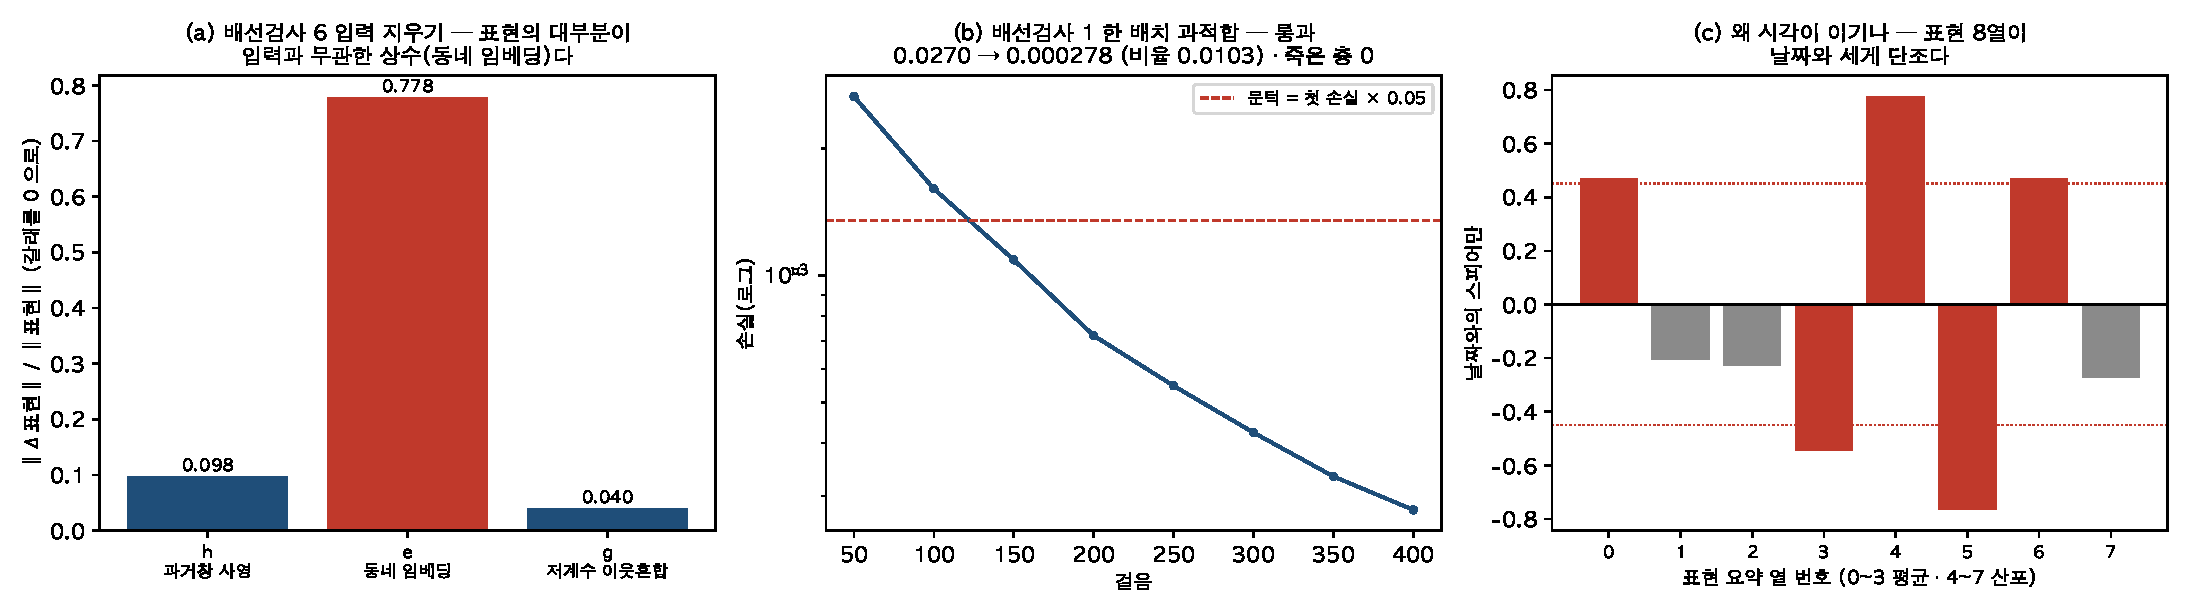
\includegraphics[width=\textwidth]{figs/fig2.pdf}
\caption{\textbf{(a)} 입력 지우기 --- 동네 임베딩을 0 으로 만들면 표현이 77.8\%
바뀌고 관측 창은 9.8\% 다. \textbf{(b)} 한 배치 과적합 통과 --- 배선은 안 끊겼다.
\textbf{(c)} 표현 8열이 날짜와 세게 단조다. 세 그림이 한 문장이다 ---
\emph{표현의 대부분은 상수이고, 시간에 따라 움직이는 작은 나머지가 달력이다.}}
\label{fig:2}
\end{figure*}

\section{0단계의 부작용이 낸 발견 --- 넷 다 재현되지 않는다}

지시는 \emph{``실제로 도는가 --- 돌려 봐라''} 였다. 돌렸더니 조각들이
\textbf{자기 산출물을 다시 썼다}. 그래서 \texttt{git diff} 가 \textbf{옛 기록값과 오늘
값의 대조표}가 됐다. \textbf{넷 다 재현되지 않는다.}

\begin{table}[h]\centering\tsize
\begin{tabular}{llrr}
\toprule
조각 & 값 & 옛 & 오늘 \\
\midrule
\texttt{shared\_encoder} & 단독 & 0.16304 & \textbf{0.20188} \\
                        & 공유 & 0.17024 & \textbf{0.18599} \\
\texttt{foundation} & 아이돌 $p$ & \textbf{0.04} & \textbf{0.06} \\
                    & 팝업 점수 & 0.7357 & 0.7163 \\
\texttt{masked\_encoder} & 도메인 수 & \textbf{10} & \textbf{12} \\
                        & 팝업 & 0.4587 & \textbf{0.1777} \\
\texttt{fewshot} & 팝업 $k{=}0$ diff & \textbf{+0.0116} & \textbf{$-$0.0231} \\
\bottomrule
\end{tabular}
\caption{0단계가 조각을 돌린 부작용. \texttt{masked\_encoder} 는 \textbf{분모가 달라졌다}
(도메인 10$\to$12) --- 그래서 종합 지표 $0.3575\to0.3174$ 는 같은 자의 변화가 아니다(조항 60).}
\label{tab:repro}
\end{table}

\claimx{\textbf{\texttt{shared\_encoder} 는 결론이 뒤집힌다.} 옛 값은 공유 $0.17024 >$
단독 $0.16304$ 로 \emph{``공유 인코더가 단독을 이긴다''} 였고 그것이 그 파일의 존재
이유였다. 오늘은 단독 $\mathbf{0.20188} >$ 공유 $\mathbf{0.18599}$ --- \textbf{부호가
뒤집힌다}. 🔴 \textbf{그런데 애초에 판정할 수 있는 값이 아니었다}: 그 파일이 스스로 적은
씨앗 SD 가 공유 $0.01778$ 인데 두 팔의 차는 $0.0072$ --- \textbf{차가 씨앗 SD 의
0.41배}다. docstring 은 \emph{``노트 14에서 씨앗 SD 가 효과의 4--5배라 아무것도 판정할
수 없었다''} 를 인용해 놓고, \textbf{적기만 하고 판정에 쓰지 않았다}.}
{같은 씨앗 다섯으로 오늘 다시 돌렸을 때 옛 값이 나오면 이 주장은 틀린다.}

\claimx{\textbf{그리고 씨앗 잡음이 아니다 --- 오늘 두 번 돌려 비트 동일하다.}
19:50 과 20:20 의 두 실행이 단독·공유·선형·\textbf{씨앗별 값까지 전부 같다}. 그러므로
기록값과의 차이는 \textbf{밑자료나 코드가 바뀐 것}이다(원인은 \emph{안 갈랐다}).
게다가 \textbf{공유 팔의 씨앗 다섯이 $+0.0922$부터 $+0.2409$까지 흩어진다}
(범위 $0.1487$ · SD $0.0519$) --- 두 팔의 차 $0.0159$ 의 \textbf{9.4배}다.
그리고 그 실행의 요약이 스스로 적는다: 단독은 선형 기준선보다 $-0.1005$
(씨앗 SD 의 \textbf{9.46배}), 공유는 $-0.1163$(2.24배) --- \textbf{두 신경망 인코더가
선형에 크게 진다}. 다만 그 선형 값 자체가 오버플로 위에서 나온다.}
{셋 중 하나라도 오늘 다시 돌려 다른 값이 나오면 「비트 동일」 주장은 틀린다.}

\claimx{\textbf{옛 논문의 그림이 살아 있는 파일을 가리키고 있었다.}
\texttt{paper/figs.py:1320,1347} 의 \texttt{fig\_foundation}(노트 14 주장 1)이
\texttt{data/state/foundation.json} 을 \emph{빌드할 때} 읽는다. 그 파일이 오늘 바뀌었으므로
\textbf{그 옛 논문을 다시 빌드하면 그림의 숫자가 조용히 바뀐다} --- 하필 바뀐 것이
\textbf{유일하게 유의했던 아이돌 $p=0.04 \to 0.06$} 이다. \textbf{죽은 숫자의 거울상}이다.}
{\texttt{figs.py} 가 실제로는 스냅샷을 읽고 있었다면 틀린다 --- 확인했다. 경로 하나이고
스냅샷이 없다.}

\claimx{\textbf{\texttt{state/masked\_encoder.py} 의 의존물이 저장소 밖에 있다.}
\texttt{masked\_encoder.py:144--145} 가
\texttt{sys.path.insert(0, "/Users/ax/.claude/jobs/a5c89f96/tmp")} 뒤
\texttt{from prior\_hit import REC, cols} 를 한다. 그 파일은 \textbf{2026-07-29 자
스크래치패드}(6,539바이트 · 버전관리 밖)이고 \textbf{반입만으로 저장소에 쓴다}
(\texttt{prior\_hit.py:155} 가 \texttt{data/state/prior\_hit.json} 에 \texttt{json.dump}).
🔴 티처 \#4 의 \emph{``규약 하나와 판정 13개를 낳은 코드가 스크래치패드에만 있었다''} 가
\textbf{아직 살아 있다.}}
{그 스크래치패드가 지워진 뒤에도 \texttt{masked\_encoder} 가 돌면 틀린다.}

🔴 \textbf{그래서 아키텍처 사다리를 이 조각들 위에 올리면 안 된다} --- L0 기준선으로
인용할 수 있는 값이 넷 다 없다. 그리고 일반화가 하나 남는다:
\texttt{data/state/*.json} 안에 \textbf{``다시 돌리면 덮이는 것''}과
\textbf{``판정의 증거로 인용되는 것''}이 \emph{같은 디렉터리에 섞여 있고},
\textbf{어느 것이 인용 중인지 아무도 세어 본 적이 없다.}

\section{남은 것}

\begin{enumerate}\setlength\itemsep{1pt}
\item \textbf{위약을 12뽑기로} --- F4 가 널 폭인지 교란인지 가른다. 제일 싸고 제일 먼저다.
\item \textbf{퇴화 제외와 시각 통제를 사전등록해서} 다시 --- 오늘 것은 사후다.
\item \textbf{사다리를 장 학습 과제로 옮긴다}(관측 143,892). 판 유보에서는 9,476 군집이 필요하다.
\item \textbf{동네 임베딩 재학습 대조} --- 상수가 여분인가 일을 하는가.
\item \textbf{$L$ 의 $b$ 항은 자료가 자라야 열린다} --- 노트 771 의 2,028행. 지금 62행.
\item \textbf{다리를 하나라도 놓는다} --- 두 인코더를 함께 반입하는 파일이 오늘 기준 0개다.
\item \textbf{\texttt{data/state/} 를 「덮이는 것」과 「인용되는 것」으로 가른다} --- 아무도 세어 본 적이 없다.
\end{enumerate}

\end{document}
